\chapter{CellTAN: Cellular Time Activation Networks} \label{chap:chap4}

Distributed information systems characterized by time series data present various challenges, primarily due to their complex and dynamic nature. The sheer volume of data that must be processed and analyzed in real time is a significant challenge, leading to concerns over storage, computation, and scalability. Moreover, data quality issues such as missing or incomplete data and data heterogeneity arising from sourcing data from disparate sources with varying consistency and structure further exacerbate these challenges. Another critical challenge of these systems is handling the temporal aspects of time series data, requiring specialized pre-processing, feature extraction, and modeling techniques. The distributed nature of these systems further complexifies matters, with issues encompassing data synchronization and accuracy being a common concern. Furthermore, their implementation in real-world applications requires robust mechanisms for data security and privacy, which adds a layer of complexity to the design and implementation of these systems.

\begin{figure}[h!]
    \centering
    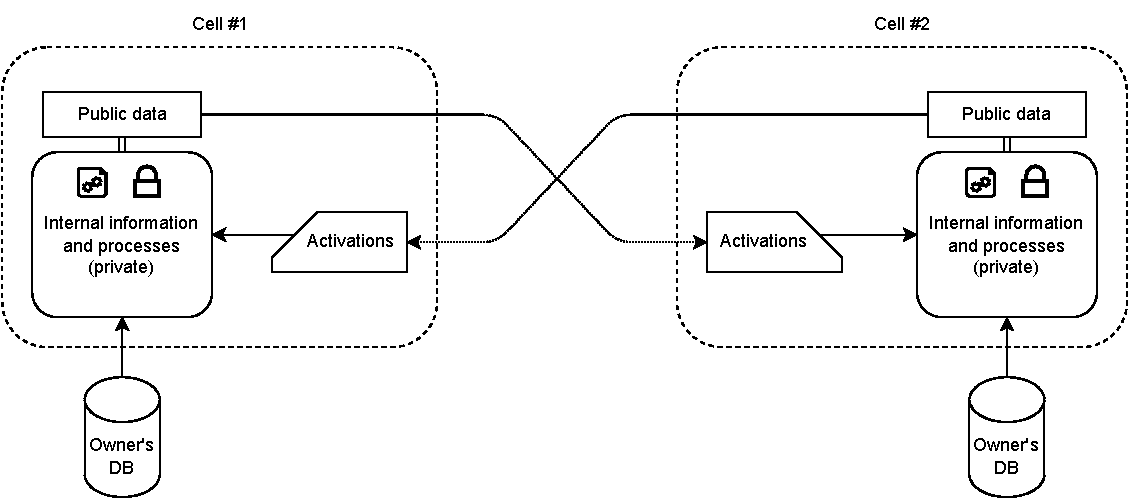
\includegraphics[width=12cm]{figures/chapter4/cell/intro.pdf}
    \caption{Simples CellTAN Network of two cells cooperating.}
    \label{fig:celltanintro}
\end{figure}

This chapter proposes a novel tool entitled CellTAN (Cellular Time Activation Network) that undertakes those challenges. CellTAN represents sparse yet interconnected components that function independently, cooperatively, and asynchronously. Inspired by other effective mechanisms like GNNs, CXNs, and Weighted Cross-Connection Networks (WCCNs), CellTAN uses a graph-like structure to represent a network of components, with nodes and connections. Following the introductory chapters, its primary purpose is to detect anomalous scenarios on PV systems. However, its generalized formulation introduces other valuable features which come naturally from fulfilling this goal. Such are state estimation, forecasting, and capturing the value in data from different PV asset owners without violating their privacy. For briefness' sake, we will the details about its benefits to be unfolded during the rest of this chapter.

Instead of tackling fault detection and classification in a classical centralized manner, which is already extensively showcased throughout the literature, this tool approaches this problem with a paradigm change: a distributed and asynchronous data coherence system. By having a virtual representation closely related to the physical form of sparse systems, relationships between components can be leveraged to assess their correct (or incorrect) operation. While initially designed for photovoltaic (PV) systems, the concepts of cells, connections, neighbors, time series, and uncertainty are universal and applicable to other fields such as biology, physics, and more. Thus, the potential for generic applicability sparks the interest to not bake specifics of PV systems directly into this tool, allowing its usage for other subjects. Figure \ref{fig:celltanintro} represents minimal scenario for a network: only two cells. It showcases some terms specific to this tool, that might be difficult to grasp at first, such as trust, events, and activations. Consequently, the glossary in \ref{sec:glossary} and detailed explanations throughout this chapter serve to clarify them.

Vast and scattered information across multiple agents is a common scenario faced by the industry of AI for energy systems, which cannot be aggregated due to privacy and confidentiality reasons. Nevertheless, its conjunction could have a lot of added value, given the similarity of certain assets: PV plants (as well as wind farms) from different owners in neighbouring geographical regions. This information-sharing potential for AI algorithms motivates the development of a mechanism that provides a way of communicating information between differently owned assets without any of the compromises above. However, and as stated before, data acquisition in PV scenario's is scarcely synchronous and might not occur in equal time resolutions for all the different components. The CellTAN addresses these issues with an instrument referred to as \textbf{Time activations}. It proposes a new way of communication that decouples from the needs of units, sampling rate, and synchronization, avoiding any resampling, normalization, or even obfuscation (to protect privacy). This mechanism is a core feature of the tool since it will be the means that will allow connecting different stakeholders' data, hence section \ref{sec:thecell} develops this matter thoroughly. Likewise, succeeding sections formulate the working of the \textbf{Cell} and its interactions within the network. Since it is the core component, understanding its behavior is crucial for a complete understanding of the tool.

\section{Glossary} \label{sec:glossary}


\begin{itemize}
    \item \textbf{Knowledge base}: Refers to registered historical knowledge (samples) of time series variables.

    \item \textbf{Inputs}: Uniform fuzzy numbers (not necessarily, but it's the current choice) that represent one sample of the group of time series variables that define the state of a cell.

    \item \textbf{Outputs}: Similar to inputs, but obtained through mroe complex computations.

    \item \textbf{Time decay}: A process associated with increased uncertainty of variables over time.

    \item \textbf{Activations}: Timestamps of past ocurrences on a knowledge base that have a non zero value of membership against a set of recent inputs.

    \item \textbf{Events}: Occurences that the cell reports back to the hub, that in most cases are triggered by the exceeding of parametrized thresholds.

    \item \textbf{Trust}: A decimal number that represents how coherent two cells's activations are with each other. Besides its instantaneous computed value, it can also come from a cumulative computation on a defined time window.

    \item \textbf{Hub}: The central component of the cell network, which facilitates its visualization, management, and expansion. It acts as the proxy agent between the cell's communication.

\end{itemize}

\section{The Cell} \label{sec:thecell}

\subsection{Principles}

A cell is an independent entity composed of \textbf{data} and \textbf{processes}. The idea is to abstract fundamental system components (e.g. inverters, MPPT's) into this virtual entity. With an added intelligence layer and featuring a few different processes, it assesses its current state based on all available internal and external information, adding value to the existing data acquisition and monitoring systems. As an individual part of the system, it follows a set of rules that define its intrinsic and extrinsic behavior. These rules address data privacy, request boundaries, and real-world operational limitations.

\paragraph*{Independence} During operation, independence on neighbors or other network entities for continuous processing of outputs results in a more robust system and increases availability. Thus, given any connection cutoffs, the cell shall be unbothered by its surroundings and continue operating in an isolated state. Isolation is not preferred, but enduring it until outside contact is re-established avoids shutdown and startup procedures.

\paragraph*{Selfish Computations} The cell is selfish in that it will not perform any computations based on the request of others. This aspect creates a fundamental layer of protection against overloading the infrastructure in which it is deployed, which also increases availability.

\paragraph*{Selfless Data} Although selfish in computations, the cell shall provide access to select data valuable to the network. However, public data shall not compromise the cell's privacy (more on this later).

\subsection{Processes and Data}

\begin{figure}[h!]
    \centering
    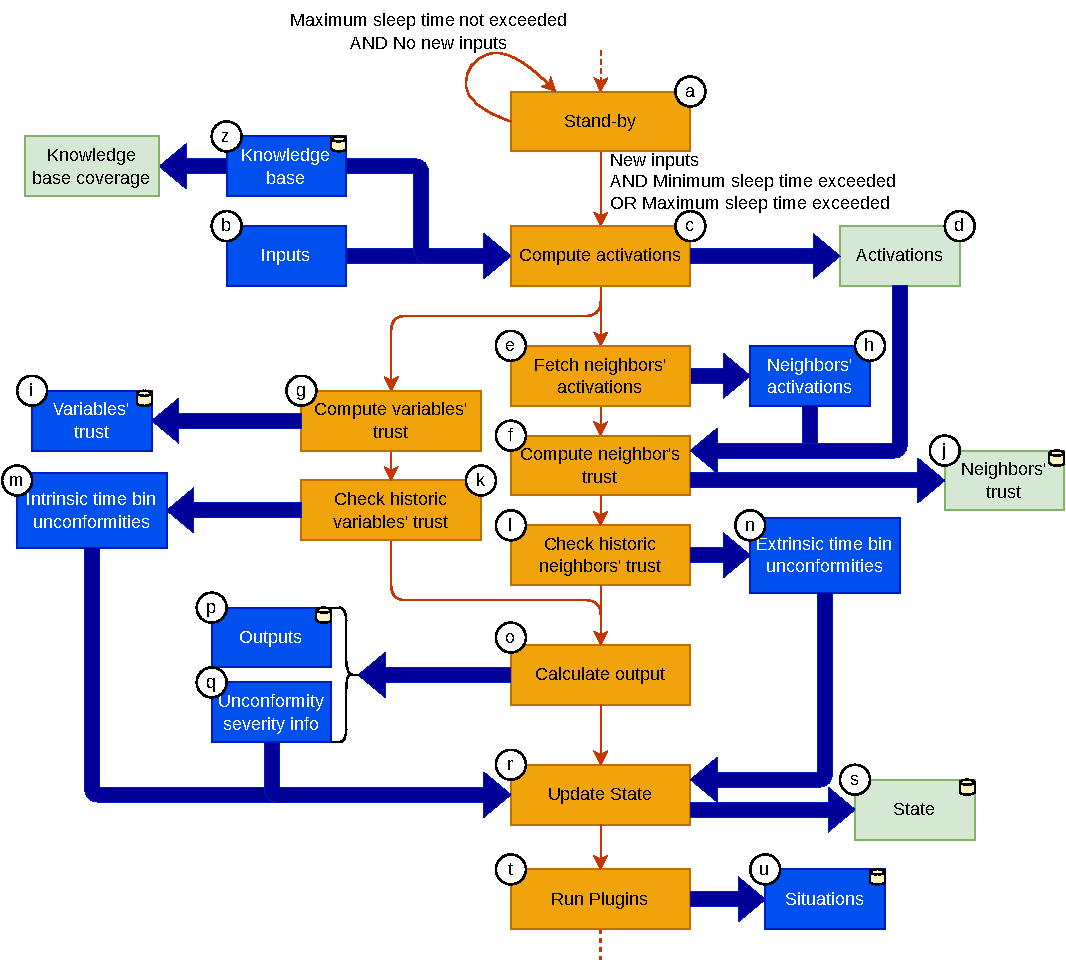
\includegraphics[width=12cm]{figures/chapter4/cell/processes.pdf}
    \caption{Cell's core main loop of processes.}
    \label{fig:cellprocesses}
\end{figure}

\subsection{Inputs and Outputs}

The cell has inputs and outputs. Both are a view of the values that define its variables at a given timestamp, which is continuously rolling. While inputs are directly associated with raw sampled data from the system (injected by the owner), outputs are a byproduct of internal processes. The latter should present more accurate information since it is based on internal and external information (ideally).
Representing the cell's variables in a fuzzy (or probabilistic) manner can better capture the inherent uncertainty in time series data. For the cell's inner workings, we chose that inputs and outputs are not represented by crisp values but rather by classical sets. However, they are not limited to sets; fuzzy numbers or probability distributions could represent them. Thus, inputs and outputs may be characterized by:

\begin{itemize}
    \item Classical set: simple uncertainty band (e.g. uncertainty up, down, relative, etc);
    \item Fuzzy number: generalized fuzzy number representation \cite{Zhang2019} (e.g. triangular fuzzy number (a,b,d;h));
    \item Probability distribution: the distribution's characteristics (e.g. mean ($\mu$) and standard deviation ($\delta$) for Gaussian, mean rate of occurence ($\lambda$) for Poisson, etc.);
\end{itemize}

\begin{figure}[h!]
    \centering
    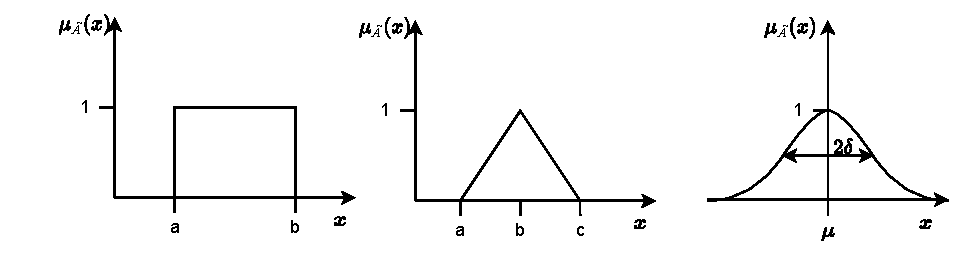
\includegraphics[width=15cm]{figures/chapter4/cell/classic_fuzzy_gaussian.pdf}
    \caption{Classical set, triangular fuzzy number and gaussian distributions and the associated membership function.}
    \label{fig:classicfuzzygaussian}
\end{figure}

Thanks to this representation, both inputs and outputs can be subject to a process named \textbf{time decay}, which ensure that the passage of time negatively affects uncertainty (more on section \ref{subsec:timedecay}).


\subsection{Time decay} \label{subsec:timedecay}

In real-world dynamic systems that involve data acquisition, the certainty of the data collected tends to fade over time due to the nature of the data acquisition process. Typically, the most recent data is the most accurate representation of the system's current state, and as time elapses, the accuracy of previous data points decreases. This occurs naturally due to various factors such as environmental changes, equipment degradation, or other system's dynamics. As a result, it is crucial to consider the time dimension when analyzing dynamic systems and to develop methods that can account for the decay in data certainty over time.

Towards considering the time dimention for the current state of a cell, we formulate a \textbf{time decay} method to ensure a more truthful and reliable assessment of its current state. During the standby stage, this process ensures that the inputs and outputs suffer an increase in uncertainty, which is has different side effects depending on what represents them (classical set, fuzzy number or probability distribution).

Consider the following example of converting a crisp value and uncertainty to a set:

$$x = 5 \pm 1 \rightarrow [5-1, 5+1] = [4, 6]$$

To simulate the increase in uncertainty over time, we can apply the following formula to each bound:

\begin{equation}
lower = lower - (lower - minimum) \times \frac{age}{decay}
\end{equation}

\begin{equation}
upper = upper + (maximum - upper) \times \frac{age}{decay}
\end{equation}

\begin{figure}[h!]
    \begin{floatrow}
    \capbtabbox{%
    \resizebox{4cm}{!}{%
        \begin{tabular}{|l|l|l|}
            \hline
            $x_{min}$   & $x_{max}$   & decay (s) \\ \hline
            0       & 10      & 10        \\ \hhline{===}
            $x_{lower}$ & $x_{upper}$ & age (s)   \\ \hline
            4.000   & 6.000   & 0.000     \\ \hline
            3.600   & 6.400   & 1.000     \\ \hline
            2.880   & 7.120   & 2.000     \\ \hline
            2.016   & 7.984   & 3.000     \\ \hline
            1.210   & 8.790   & 4.000     \\ \hline
        0.605   & 9.395   & 5.000     \\ \hline
        0.242   & 9.758   & 6.000     \\ \hline
        0.073   & 9.927   & 7.000     \\ \hline
        0.015   & 9.985   & 8.000     \\ \hline
        0.001   & 9.999   & 9.000     \\ \hline
        0.000   & 10.000  & 10.000    \\ \hline
    \end{tabular}%
    }
    }{%
    \caption{Parameters and values of $x_{lower}$ and $x_{upper}$ varying with age.}%
    \label{tab:timedecay}
    }
    \ffigbox{%
    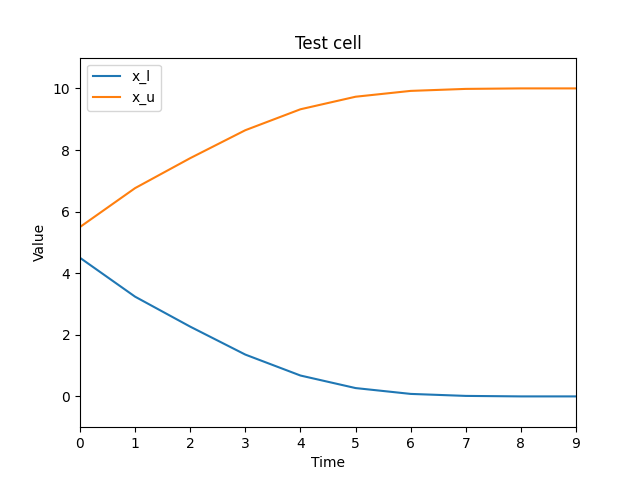
\includegraphics[width=9cm]{figures/chapter4/cell/time_decay.png}%
    }{%
      \caption{Visualization of $x_{lower}$ and $x_{upper}$ expanding through time.}%
      \label{fig:timedecay}
    }
    \end{floatrow}
    \end{figure}

% \begin{figure}[h!]
%     \centering
%     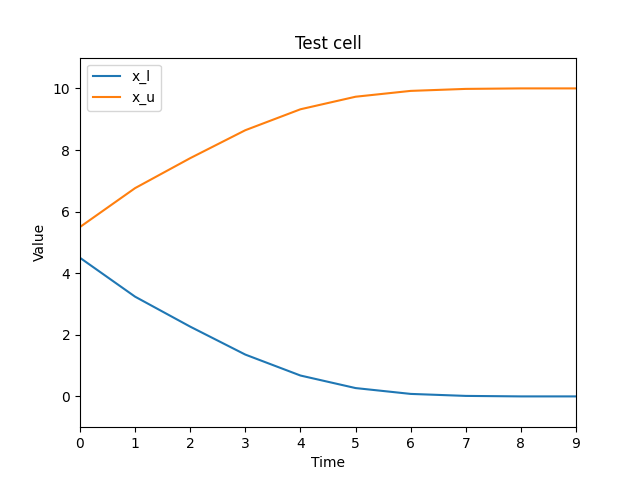
\includegraphics[width=10cm]{figures/chapter4/cell/time_decay.png}
%     \caption{Time decay.}
%     \label{fig:timedecay}
% \end{figure}

% TODO
Table \ref{tab:timedecay} and figure \ref{fig:timedecay} represent the expansion of the set throughout a period of time equal to the decay parameter (ten seconds). We can observe an exponential decay caused by the simultaneous variation of age and difference between bounds and maximum/minimum.

\subsection{Temporal similarity extraction} \label{subsec:tempsim}

Temporal similarity extraction the process of identifying recurring patterns in time series data. It involves the identification of past instances where the current state is observed to extract useful information about the system's behavior over time. By identifying historical periods with similar states, temporal similarity extraction can help assess the current state or predict future trends. This technique is common in statistics, for purposes such as estimation and forecasting.

Using sets or probability distributions to filter historical data is one approach to simplify the process of temporal similarity extraction in multivariate time series data, while also making it more robust against noisy or incomplete data. This approach assigns membership values to each data point in the time series based on the corresponding set (or distribution) generated from the current cell inputs, and by eliminating samples past a certain threshold we can generate outputs. This is one of the reasons for deciding to represent the inputs and outputs of the cell in a fuzzy manner. 

The proposal for similarity extraction in the cell consists of receiving new values (inputs) for the cell's variables from a data source (sensors or other data acquisition equipment, calculations, forecasting, etc.), generating a classical set, fuzzy number, or probability distribution from them, and then applying the bounds/membership function or probability density function to the knowledge base (see figure \ref{fig:solo_state_estimation}). When historical samples are associated with membership values, there may be a process for determining outputs by combining data and membership values.

The initial choice is to use classical sets since filtering history becomes trivial and efficient: restrict the knowledge base to samples where all variables belong to the corresponding interval. Generating outputs with these can be as simple as constructing new sets based on the bounds of filtered knowledge (samples with membership equal to one). When filtering historical data with two or more variables, there is a trend of narrowing down the resulting data's space due to the intersection of constraints. Therefore, this process should result in sets that are an equal or better assessment of the present state (than the sets generated by inputs). However, filtering might also result in zero samples (membership value of zero on all knowledge base's rows), which indicates not having "memory" of any similar occurrence. This zero-sample filter is an excellent indicator for potentially anomalous scenarios, primarily if we know that the knowledge base is statistically representative of the variables in the cell.

This process also makes possible for simple forecasting. Considering an offset (arbitrary number of rows forward) in the activations, the temporal similarity extraction and computation of outputs results in future values. So, cells may either compute outputs related to the present or future. Nonetheless, this temporal shift might be difficult to achieve if data samples arrive at randomly spaced intervals of time, thus would only be straightforward for systems with time-consistent data acquisition.

The following examples consider that $t=0$ is associated with the present, and $\mu$ represents membership functions.

\paragraph{Self Similarity}
Having a knowledge base and input variables, the cell can perform intrinsic temporal similarity extraction.
Consider the a cell that is characterized by two variables, which are a function of time: $x(t)$ and $y(t)$.
Assume that, at a given instant, these are the new cell inputs:

\begin{equation}
    x(0) = 1.0 \rightarrow \mu_{x(0)}(x) =
    \begin{cases}
        1, & x \in [0.9, 1.1]    \\
        0, & x \notin [0.9, 1.1] \\
    \end{cases}
\end{equation}

\begin{equation}
    y(0) = 2.0 \rightarrow \mu_{y(0)}(y) =
    \begin{cases}
        1, & y \in [1.8, 2.2]    \\
        0, & y \notin [1.8, 2.2] \\
    \end{cases}
\end{equation}

The membership functions $\mu$ are generated considering that $x$ and $y$ are characterized by uniform and symetrical uncertainty, and that the received samples of $x(0)$ and $y(0)$ represent its median.

\begin{figure}[h!]
    \centering
    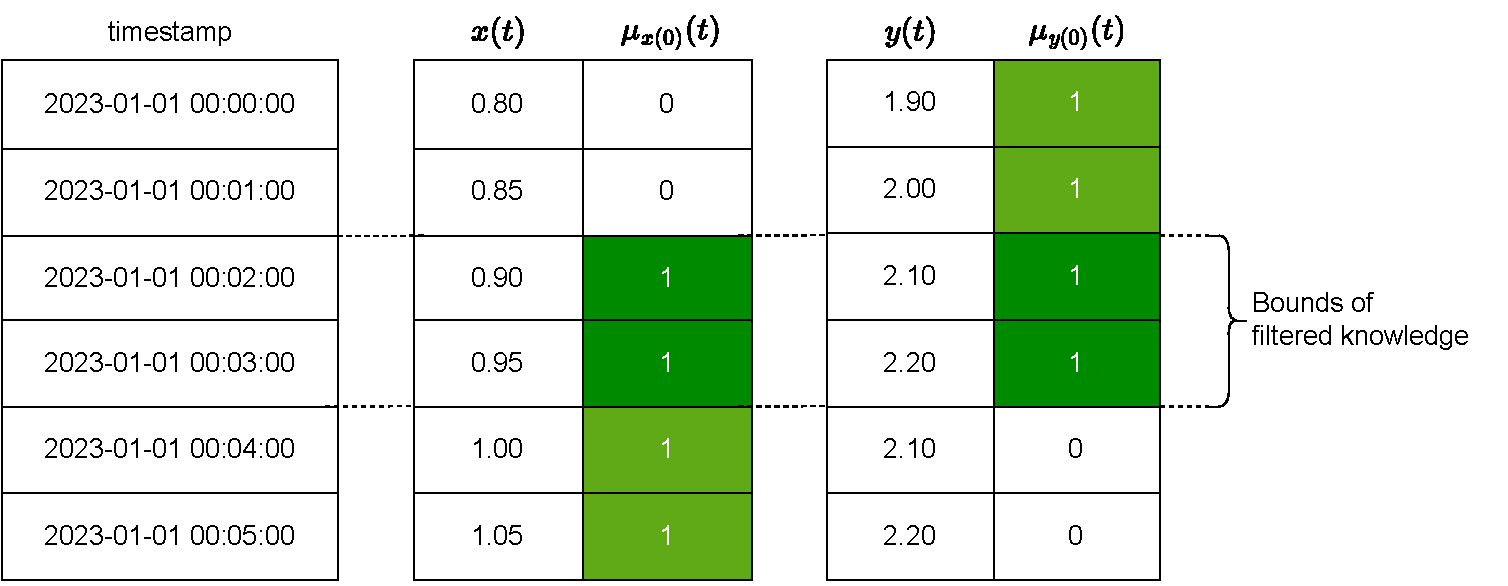
\includegraphics[width=\linewidth]{figures/chapter4/cell/solo_state_estimation.pdf}
    \caption{Visualization of a self similarity extraction example.}
    \label{fig:solo_state_estimation}
\end{figure}


With the knowledge base represented in figure \ref{fig:solo_state_estimation}, the resulting activations will be 2023-01-01 00:02:00 and 2023-01-01 00:03:00. These are the timestamps of past instances where the cell's variables have values belonging to the set generated from new inputs. Now we can also infer that the actual values of $x$ and $y$ should reside in a set constrained by the filtered historical data ($x(t)$ and $y(t)$). Therefore, the outputs based on self similarity extraction are:

\begin{equation}
    x'(0) \in [0.90, 0.95]
\end{equation}

\begin{equation}
    y'(0) \in [1.80, 2.20]
\end{equation}

These results confirm that outputs with less uncertainty are achieved, while only depending on intrinsic processes and private data.

\paragraph{Mutual Similarity}
\dots
% Capacidade de estimação de estado intrínsica + extrínsica

\subsection{Connections and Trust}

A network could not be formed without the existence of connections. Having neighbours grants the cells perform actions such as mutual similarity extraction. Besides, there can be certain indicators associates with these links, and to take advantage of sharing information with neighbours, there comes a need to have something we named \textbf{Trust}.

In order to distinguish cells, each one of them has a unique identifier, generated upon criation and independent from the cell's name. This serves to easily register cells and manage the network. Since interconnections require an agent to keep track of these id's and correctly direct traffic, we introduce a component named \textbf{Hub} for keeping track of registered cells in the network and their corresponding id's. By having a central component which provides global network visibility, connections are easier to form.


\subsection{Events}

\dots


\section{The Hub}

\dots


\section{Implementation}

% TODO: escrever sobre a concretização real destas ideias
\dots
